% Latex template: mahmoud.s.fahmy@students.kasralainy.edu.eg
% For more details: https://www.sharelatex.com/learn/Beamer

\documentclass{beamer}          % Document class

\usepackage[english]{babel}        % Set language
\usepackage[utf8x]{inputenc}      % Set encoding

\mode<presentation>            % Set options
{
  \usetheme{default}          % Set theme
  \usecolortheme{default}         % Set colors
  \usefonttheme{default}          % Set font theme
  \setbeamertemplate{caption}[numbered]  % Set caption to be numbered
}

% Uncomment this to have the outline at the beginning of each section highlighted.
% \AtBeginSection[]
% {%   \begin{frame}{Outline}
%     \tableofcontents[currentsection]
%   \end{frame}
% }

\usepackage{graphicx}          % For including figures
\usepackage{booktabs}          % For table rules
\usepackage{hyperref}          % For cross-referencing
\usepackage{tikz}            % For diagrams
\usetikzlibrary{positioning}     % For relative node placement

\title{Some Statistics and Bootstrap Methods}  % Presentation title
\author{aled}                % Presentation author
\institute{SDE seminars}          % Author affiliation
\date{\today}                  % Today's date

\begin{document}

% Title page
% This page includes the informations defined earlier including title, author/s, affiliation/s and the date
\begin{frame}
  \titlepage
\end{frame}

% Outline
% This page includes the outline (Table of content) of the presentation. All sections and subsections will appear in the outline by default.
\begin{frame}{Outline}
  \tableofcontents
\end{frame}

% The following is the most frequently used slide types in beamer
% The slide structure is as follows:
%
%\begin{frame}{<slide-title>}
%  <content>
%\end{frame}

\section{Statistics Foundations}

\begin{frame}{Foundations of Statistics}
  \textit{Statistical inference} == learning in computer science. \\

  we use data to infer the distribution that this data comes from

  \boxed{\text{given a sample } X_1 \hdots X_n \sim F, \text{ how do we learn something about } F?}

  \vspace{0.5cm}
  \centering
  to answer this, we first need to choose what kind of \textit{model} for $F$ we're willing to assume

  \vspace{0.3cm}
  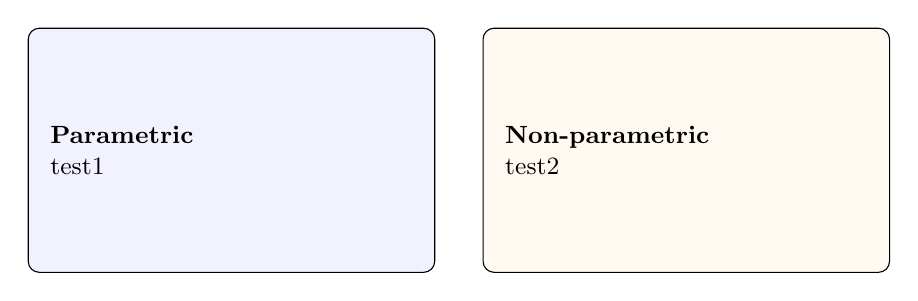
\begin{tikzpicture}[
      box/.style={draw, rounded corners, align=left, text width=4.6cm, minimum height=3.1cm, inner sep=8pt, font=\small}
    ]
    \node[box, fill=blue!5] (param) {
      \textbf{Parametric} \\

      test1
    };
    \node[box, fill=orange!5, right=0.6cm of param] (nonparam) {
      \textbf{Non-parametric} \\

      test2
    };
  \end{tikzpicture}

\end{frame}

\begin{frame}{What is Statistical Inference?}
  Inferential problems can be classified into three main categories:

  \vline

  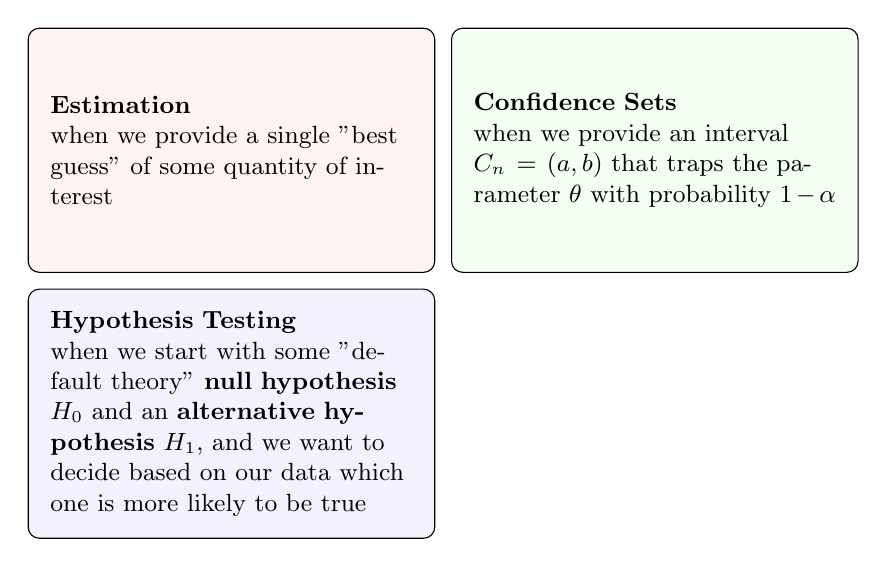
\begin{tikzpicture}[
      box/.style={draw, rounded corners, align=left, text width=4.6cm, minimum height=3.1cm, inner sep=8pt, font=\small}
    ]
    \node[box, fill=red!5] (estimation) {
      \textbf{Estimation} \\

      when we provide a single "best guess" of some quantity of interest
    };
    \node[box, fill=green!5, right=0.2cm of estimation] (confidence) {
      \textbf{Confidence Sets} \\

      when we provide an interval $C_n = (a, b)$ that traps the parameter $\theta$ with probability $1 - \alpha$
    };
    \node[box, fill=blue!5, below=0.2cm of estimation] (hypothesis) {
      \textbf{Hypothesis Testing} \\

      when we start with some "default theory" \textbf{null hypothesis} $H_0$ and an \textbf{alternative hypothesis} $H_1$, and we want to decide based on our data which one is more likely to be true
    };
  \end{tikzpicture}x
\end{frame}

\begin{frame}{More About Confidence Sets}
  We have an interval  $C_n = (a, b)$ where $a = a(X_1, \hdots, X_n)$ and $b = b(X_1, \hdots, X_n)$ are functions of the data such that
  \begin{equation}
    \mathbb{P}_\theta(\theta \in C_n) = 1 - \alpha, \text{for all } \theta \in \Theta.
  \end{equation}

  When $\theta$ is a vector than $C_n$ is a neighborhood called a \textbf{Confidence Set}.

  \begin{alertblock}{Warning \#1}
    $C_n$ is \textbf{random} and $\theta$ is \textbf{fixed}.
  \end{alertblock}
  \begin{alertblock}{Warning \#2}
    There is so much confusion about how to interpret the confidence interval.
  \end{alertblock}

\end{frame}

% \begin{frame}{Slide with two columns}
%   \begin{columns}
%     \column{.5\textwidth}
%     Text goes in first column.

%     \column{.5\textwidth}
%     Text goes in second column
%   \end{columns}
% \end{frame}

\section{Bootstrap Methods: why we need it?}

\begin{frame}{Bootstrap Methods}
  The \textbf{bootstrap} is a method for estimating \textit{standard errors} and \textit{computing
  confidence intervals} for the \textit{statistic}. Kinda \textbf{estimator for the estimator}.\\

  \vspace{0.4em}

  Suppose we have a single sample $X_1 \hdots X_n \sim F$ and statistic $T_n = T(X_1 \hdots X_n)$.
  And we wish to know for example a variance of our statistic.

  \vspace{0.4em}

  \begin{center}
    \fbox{\parbox{0.85\linewidth}{\centering
        idea has two steps:
        \begin{enumerate}
          \item \textbf{Estimate} $\mathbb{V}_{F}(T_n)$ with $\mathbb{V}_{\hat{F_n}}(T_n)$ (called \textbf{plug-in});
          \item \textbf{Approximate} $\mathbb{V}_{\hat{F_n}}(T_n)$ using \textbf{simulation};
        \end{enumerate}
    }}
  \end{center}

  \begin{exampleblock}{btw}
    now for out statistic we can calculate (almost) whatever we want:
    bias,  variance,  MSE, build confidential intervals and so on.
  \end{exampleblock}

\end{frame}

\subsection{Classic Bootstrap (in Deep)}

\begin{frame}{{\renewcommand{\thefootnote}{\fnsymbol{footnote}} Classic Bootstrap \footnote{\textit{empirical bootstrap} / \textit{nonparametric bootstrap} / \textit{Efron's bootstrap}}}: how does it works?}

  \begin{figure}
    \centering
    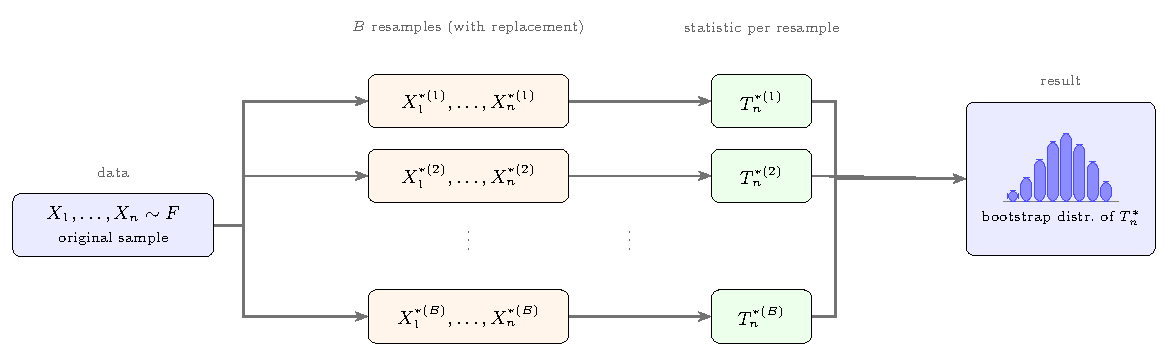
\includegraphics[width=1\textwidth]{figures/bootstrap_scheme.pdf}
  \end{figure}

  \begin{exampleblock}{btw}
    bootstrap is the method to get an \textit{ensemble} from a single process realization.
  \end{exampleblock}

\end{frame}

\begin{frame}{Classic Bootstrap: how does it works?}
  Our goal is to estimate the error of sample \textit{median} (or some other \textit{statistic}) and construct the corresponding confidence interval. \\

  \vspace{1em}

  Assume we have a sample $X_1, \hdots, X_n$ from an unknown distribution $F$ and let $M_n = \text{med}\{X_1 \hdots X_n\}$. \\

  \vspace{1em}

  Now let's sample with replacement $B$ times and so obtain \textit{bootstrap samples}:
  \begin{align*}
    X_1^{*(1)} \hdots X_n^{*(1)} \\
    X_1^{*(2)} \hdots X_n^{*(2)} \\
    \hdots \\
    X_1^{*(B)} \hdots X_n^{*(B)}
  \end{align*}
\end{frame}

\begin{frame}{Classic Bootstrap: how does it works?}
  We have $B$ \textit{bootstrap samples} and we can compute the corresponding \textit{bootstrap medians}:
  \begin{align*}
    M_n^{*(1)} = \text{med}\{X_1^{*(1)} \hdots X_n^{*(1)}\} \\
    M_n^{*(2)} = \text{med}\{X_1^{*(2)} \hdots X_n^{*(2)}\} \\
    \hdots \\
    M_n^{*(B)} = \text{med}\{X_1^{*(B)} \hdots X_n^{*(B)}\}
  \end{align*}

\end{frame}

\begin{frame}{Classic Bootstrap: how does it works?}
  And now we can compute some really cool things:
  \begin{enumerate}
    \item \textbf{Bootstrap estimate of the variance}:
      \begin{equation*}
        \widehat{\mathbb{V}}_B(M_n) = \frac{1}{B - 1}\sum_{b=1}^{B}(M_n^{*(b)} - \overline{M_B^*})^2, \quad \overline{M_B^*} = \frac{1}{B}\sum_{b=1}^{B}M_n^{*(b)}
      \end{equation*}
    \item \textbf{Bootstrap estimate of the MSE}:
      \begin{equation*}
        \widehat{\text{MSE}}_B(M_n) = \frac{1}{B}\sum_{b=1}^{B}(M_n^{*(b)} - M_n)^2
      \end{equation*}
    \item \textbf{Bootstrap confidence interval}: $1 - \alpha$ confidence interval of the population median:
      \begin{equation*}
        C_\pm = M_n \pm z_{1 - \alpha/2}\sqrt{\widehat{\mathbb{V}}_B(M_n)}.
      \end{equation*}
  \end{enumerate}
\end{frame}

\begin{frame}{Classic Bootstrap: why does it works?}
  Little weird, isn't it? We generate "new" datapoints from the original single sample we have. Does it make sense? \textbf{Under some conditions -- yes}! \\

  \vspace{1em}

  Let's be more specific: our sample $X_1, \hdots, X_n \sim F$ for some unknown distribution $F$. Every statistic $T_n = T(X_1, \hdots, X_n)$ will depend on the CDF $F$ and the sample size $n$, median too. \\

  \vspace{1em}

  So we may write a CDF for the median:
  \begin{equation}
    F_{M_n}(x) = \Psi(x; F, n),
    \label{approxmed}
  \end{equation}
  where $\Psi$ is some really complicated function (but smooth with respect to F -\_-). \\

\end{frame}

\begin{frame}{Classic Bootstrap: why does it works?}
  When we building our bootstrap samples, what is the distribution we are sampling from?

  \vspace{1em}

  Let write a EDF (Empirical Distribution Function) for our original sample:
  \begin{equation}
    \widehat{F}_n(x) = \frac{1}{n}\sum_{i=1}^{n}\mathbb{I}(X_i \leq x).
  \end{equation}

  Now generate \textmd{IID} $Z_1, \hdots, Z_n$ sample from $\widehat{F}_n$. \\

  For each $Z_j, \; j = \overline{1, n}$ we have:
  \begin{equation}
    \mathbb{P}(Z_j = X_i) = \frac{1}{n}, \quad i = \overline{1, n}.
  \end{equation}

  but wait... this sample is  exactly a \textit{sample generated by sampling with replacement from the original} $X_1, \hdots, X_n$.

\end{frame}

\begin{frame}{Classic Bootstrap: why does it works?}
  Thus, we can obtain that each bootstrap sample is an \textmd{IID} sample from $\widehat{F}_n$:

  \begin{align*}
    X_1^{*(1)} \hdots X_n^{*(1)} \sim \widehat{F}_n \\
    X_1^{*(2)} \hdots X_n^{*(2)} \sim \widehat{F}_n \\
    \hdots \\
    X_1^{*(B)} \hdots X_n^{*(B)} \sim \widehat{F}_n
  \end{align*}

  We can also write a CDF for each bootstrap median according to \eqref{approxmed}:
  \begin{equation}
    F_{M_n^{*(1)}}(x) = \hdots = F_{M_n^{*(B)}}(x) = \Psi(x; \widehat{F}_n, n).
  \end{equation}
\end{frame}

\begin{frame}{Classic Bootstrap: why does it works?}
  We know that $\widehat{F}_n \approx F$ with $n \rightarrow  \infty$ and remember that $\Psi$ is \textit{smooth} with respect to $F$, so we can conclude that:
  \begin{align}
    &\widehat{F}_n \approx F \\
    &\implies \Psi(x; \widehat{F}_n, n) \approx \Psi(x; F, n) \\
    &\implies F_{M_n^{*(b)}}(x) \approx F_{M_n}(x)
  \end{align}

  \begin{center}
    \fbox{\parbox{0.85\linewidth}{\centering
        the CDF of a bootstrap median $F_{M_n^{*(b)}}(x)$ approximates the CDF of the true median $F_{M_n}(x)$
    }}
  \end{center}
\end{frame}

\begin{frame}{Classic Bootstrap: why does it works?}

  This has many implications, for example, we can now estimate the variance of the median:
  \begin{equation*}
    \mathbb{V}(M_n) \approx \mathbb{V}(M_n^{*(b)}) \approx \widehat{\mathbb{V}}_B(M_n).
  \end{equation*}

  Also we can \textbf{generalize} this statements to many other statistics:
  \begin{itemize}
    \item quantiles;
    \item skewness (related to $\mathbb{E}(X^3)$);
    \item kurtosis (related to $\mathbb{E}(X^4)$);
    \item $\hdots$
  \end{itemize}

\end{frame}

\begin{frame}{Classic Bootstrap: when it does not works?}
  $X_1 \hdots X_n \sim \text{Uni}[0, 1]$ and statistic $M_n = \min{\{X_1 \hdots X_n\}}$.  It's known that $n M_n \sim \text{Exp}(1)$.

  Let's do the staff: $X_1^* \hdots X_n^*$ and $M_n^* = \min{\{ X_1^* \hdots X_n^* \}}$.

  The bootstrap minimum sits on an observed point $M_n$ with probability:
  \begin{align*}
    &\mathbb{P}(X_i^* = M_n) = \frac{1}{n}, \\
    &\mathbb{P}(M_n^* = M_n) \\
    & = 1 - \mathbb{P}(\text{none of } X_1^* \hdots X_n^* \text{ select } M_n) = 1 - \left( 1 - \frac{1}{n} \right)^n \approx 1 - e^{-1}.
  \end{align*}

  $\approx 63\%$ of bootstrap replicas return \textit{exactly} the sample
  minimum: the bootstrap distribution is discrete and piles mass on one point,
  while the true law of $n M_n$ is continuous ($\mathrm{Exp}(1)$).

  \begin{center}
    \fbox{\parbox{0.85\linewidth}{\centering
        extremes of $\widehat{F}_n$ do not mimic extremes of $F$.
    }}
  \end{center}

\end{frame}

\begin{frame}{Classic Bootstrap: when it does not works?}
  \begin{figure}
    \centering
    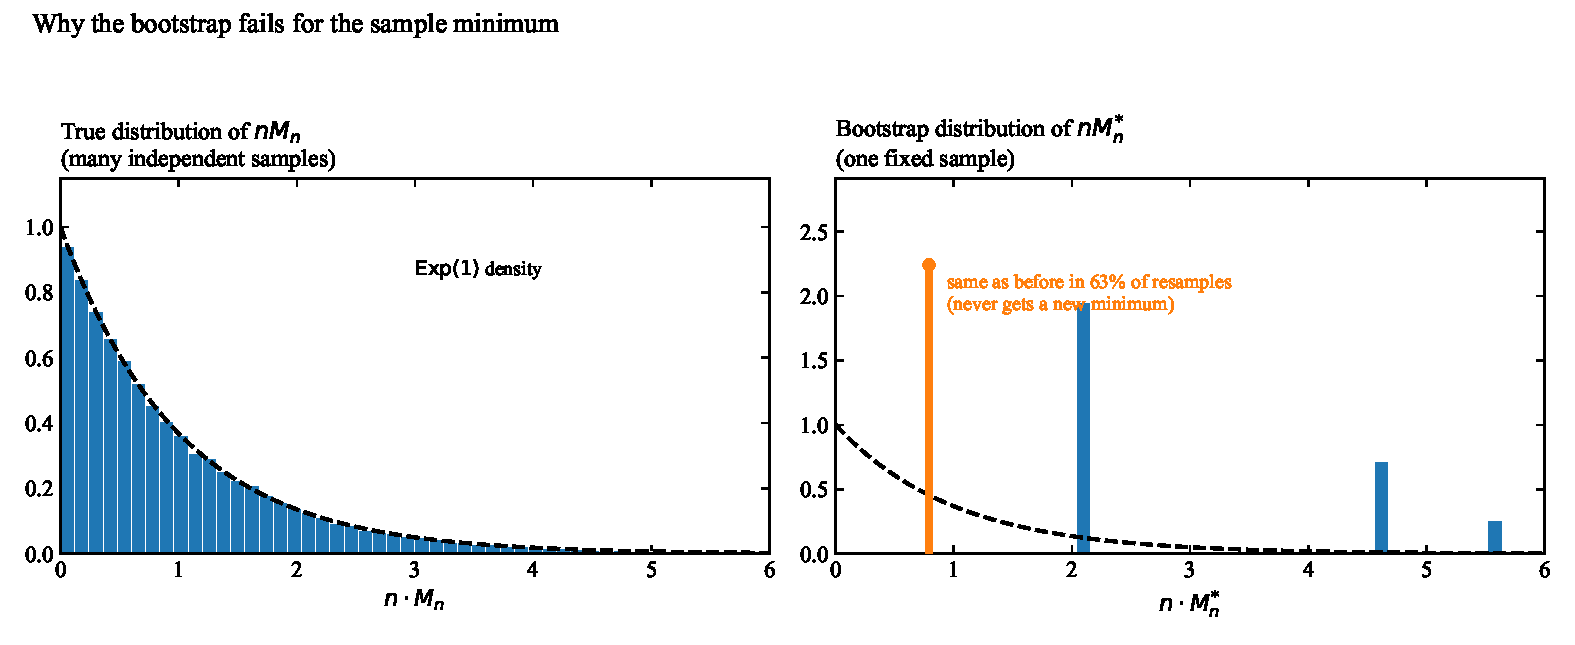
\includegraphics[width=1\textwidth]{figures/bootstrap_failure_plot.pdf}
  \end{figure}
\end{frame}

\subsection{Bootstrap Family}

\begin{frame}{Bootstrap Family}
  \begin{columns}[t]

    \begin{column}{0.5\textwidth}
      What we covered is the \textbf{classic} recipe. Around it -- a whole family,
      each member relaxing a different assumption:
    \end{column}

    \begin{column}{0.5\textwidth}
      \vspace{-3em}
      \begin{figure}
        \centering
        
\includegraphics[width=0.5\textwidth]{figures/family.png}
      \end{figure}
    \end{column}
  \end{columns}

  \vspace{-1em}

  \begin{center}
    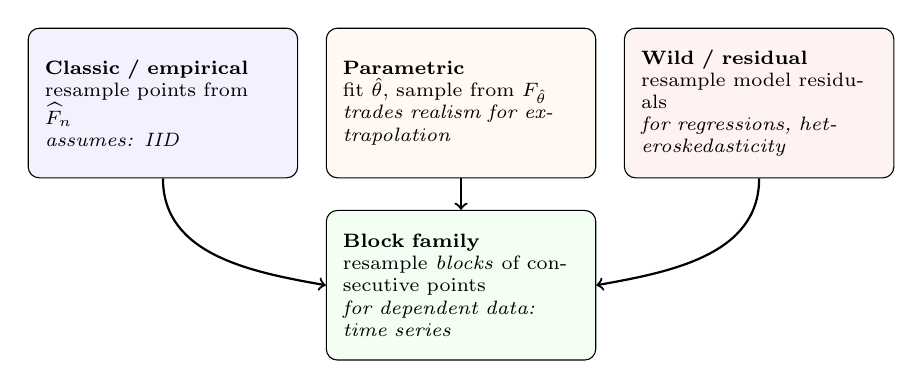
\begin{tikzpicture}[
        box/.style={draw, rounded corners, align=left, text width=3cm,
        minimum height=1.9cm, inner sep=6pt, font=\scriptsize}
      ]
      \node[box, fill=blue!5] (classic) {
        \textbf{Classic / empirical} \\
        resample points from $\widehat{F}_n$ \\
        \textit{assumes: IID}
      };
      \node[box, fill=orange!5, right=0.35cm of classic] (param) {
        \textbf{Parametric} \\
        fit $\hat\theta$, sample from $F_{\hat\theta}$ \\
        \textit{trades realism for extrapolation}
      };
      \node[box, fill=red!5, right=0.35cm of param] (wild) {
        \textbf{Wild / residual} \\
        resample model residuals \\
        \textit{for regressions, heteroskedasticity}
      };
      \node[box, fill=green!5, below=0.4cm of param] (block) {
        \textbf{Block family} \\
        resample \textit{blocks} of consecutive points \\
        \textit{for dependent data: time series}
      };
      \draw[->, thick] (classic.south) to[out=-90, in=170] (block.west);
      \draw[->, thick] (param.south) -- (block.north);
      \draw[->, thick] (wild.south) to[out=-90, in=10] (block.east);
    \end{tikzpicture}
  \end{center}

  \footnotesize
  Same \textbf{plug-in} principle everywhere; the difference is \textbf{what} we treat
  as the exchangeable unit and \textbf{where} the randomness is injected.
\end{frame}

\subsection{Block Bootstrap}

\begin{frame}{Today: the Block Bootstrap}
  Why this member of the family? Because of \textbf{our} data. \\

  \vspace{0.8em}
  Financial returns violate the IID assumption in a specific way:
  \begin{itemize}
    \item autocorrelation of $r_t$ is $\approx 0$ --- looks IID at first glance...
    \item ...but autocorrelation of $r_t^2$ persists for weeks:
      calm and stormy periods come in \textbf{streaks}
      (volatility clustering);
    \item pool metrics (fees, impermanent loss) are functionals of the
      \textit{path} --- they feel the streaks, not just the histogram
      of returns.
  \end{itemize}

  \vspace{0.8em}
  \begin{center}
    \fbox{\parbox{0.88\linewidth}{\centering
        Naive bootstrap destroys the streaks $\Rightarrow$ underestimates risk. \\
        \textbf{Part II:} resample blocks, keep the streaks ---
        and what this buys a risk team.
    }}
  \end{center}
\end{frame}

\begin{frame}{Slide with references}
  % This is to reference a figure (Figure \ref{fig:figure1})\\
  % This it to reference a table (Table \ref{tab:table1})\\
  This is to cite an article \cite{Ahmed2018a}\\
  This is to add an article to the references without mentioning in the text \nocite{Ahmed2018a}\\
\end{frame}

\section{References}
% Adding the option 'allowframebreaks' allows the contents of the slide to be expanded in more than one slide.
\begin{frame}[allowframebreaks]{References}
  \bibliographystyle{apalike}
  \tiny\bibliography{references}
\end{frame}

\end{document}